\chapter{Application to Neural Spiking Data} 
\label{chapter5-application}

\section{Outline of Methods}
We applied the theory outlined in the previous chapters to neural spiking data in which we quantified the pairwise similarity of the neural population responses to different stimuli (each represented as a high-dimensional point cloud) in terms of their geometric and topological structure. The approach of this project was to first embed the data into a lower-dimensional manifold using diffusion map and then apply the method of persistent homology to extract the topological features, specifically the persistence diagrams and the persistence barcodes. In the end, we computed the pairwise Wasserstein distance between the persistence diagrams, which measures the pairwise similarity we set out to find. 

The following flowchart shows a schematic summary of our approach.

\begin{tikzpicture}[font={\sf \small}]
 \def\smbwd{2cm}
%   \node (BNN) at (-3,0.5) [draw, terminal, minimum width=\smbwd,  fill=yellow!20, minimum height=0.5cm] {Biological Neural Networks}; 
%   \node (ANN) at (2.7,0.5) [draw, terminal, minimum width=\smbwd,  fill=yellow!20, minimum height=0.5cm] {Artificial Neural Networks}; 
  %------------
  \node (experimental) at (0,-0.5) [draw, terminal, minimum width=\smbwd,  fill=red!20, minimum height=0.5cm]{Neural population activity (lab experiments)};
%   \node (artificial) at (2.7,-1)[draw, terminal,minimum width=\smbwd,  fill=red!20, minimum height=0.5cm]{neuron output (simulations)};
  %------------
%   \node (tensors) at (0,-2) [draw, terminal, minimum width=\smbwd,  fill=red!20, minimum height=0.5cm] {Neural tensors}; 
%   %------------
  
  \node (diffusion) at (0,-2.5) [draw, process, minimum width=\smbwd, fill=blue!20, minimum height=0.7cm] {Step 1: Diffusion map};
  %------------
  
  \node (manifolds) at (0,-4.5) [draw, terminal, minimum width=\smbwd,  fill=green!20, minimum height=0.5cm] {Neural manifold};
  
   \node (persistent) at (0,-6.5) [draw, process, minimum width=\smbwd, fill=blue!20, minimum height=0.7cm] {Step 2: Persistent homology};
   
   \node (features) at (0,-8.5) [draw, terminal, minimum width=\smbwd,  fill=green!20, minimum height=0.5cm] {Topological features (persistence diagrams)};
   
   \node (wasserstein) at (0,-10.5) [draw, terminal, minimum width=\smbwd,  fill=green!20, minimum height=0.5cm] {$p$-Wasserstein distance between persistence diagrams};
  
  %------------
  
%  \path [line](BNN) -- (experimental);
%  \path [line](ANN) -- (artificial);
 \path [line](experimental) -- (diffusion) ;
%  \path [line] (artificial) -- (tensors) ;
 \path [line](diffusion) -- (manifolds);
  \path [line](manifolds) -- (persistent);
   \path [line](persistent) -- (features);
  \path [line](features) -- (wasserstein); 
 \end{tikzpicture}
 
\section{Data Collection}

The neural spiking data (\cite{dyballa_manifold_2021}) were collected from lab experiments with the setup shown in the figure below. Six different types of flow stimuli developed in \cite{visual-flow} were flashed in front of the mouse. The electrodes recorded the neural output from the mouse's retina while it viewed each flow stimuli moving in eight directions respectively. The neural recordings were encoded in peristimulus (PSTH) diagrams, each of which showed the firing rate of one neuron over time for the eight directions respectively. In the PSTH diagram the brighter pixels indicate higher firing rates.
 \begin{figure}[H]
        \centering
            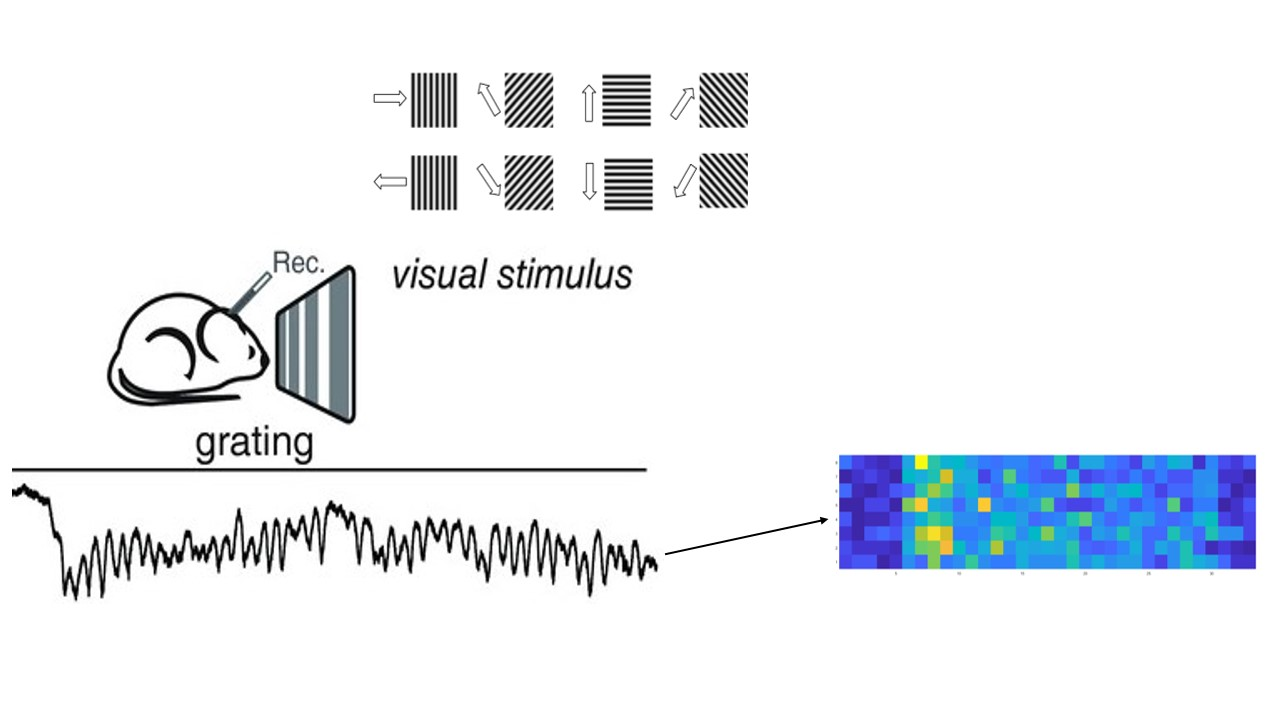
\includegraphics[width=0.55\textwidth]{figures/Slide5.jpg}
            \caption{Visualising neural data from lab experiments.}
    \end{figure}
    
\par The neural spiking data is of three dimensions: the first dimension represents the $698$ neurons; the second dimension represents the six different types of stimuli; the third dimension represents the vectorized PSTH diagrams, each of which has $8\times 33 = 264$ pixels. This gives us a $3$-way tensor:

\begin{defn}[Neural tensors]
    Suppose $\mathcal{S}$ is a set of flow stimuli $\mathcal{S} = \{s_1, s_2,\dots, s_K\}$, each moving over  $T$ time steps. The \underline{neural population response} of a set of $N$ neurons to some stimulus $s_i$ over time is $\mathcal{N} = \{\vec{n}_1, \vec{n}_2, \dots, \vec{n}_N\},$ where $\vec{n}_i \in \mathbb{R}^{T}$. 

    Each \underline{neural tensor} encodes the neural population response of $N$ neurons to $K$ flow stimuli over $T$ time steps and is thus a $3$-way $N$-by-$K$-by-$T$ tensor.
\end{defn}

With this neural spiking data set, we can create six point clouds, each corresponds to the neural population response towards one type of stimuli, which we denote as $X_1, X_2, \dots,X_6$. Each of the point cloud $X_i$ is thus represented by a matrix of dimension $698$-by-$264$, giving us a point cloud of $698$ points in $\RR^{264}$. 

\section{Step 1: Dimensionality Reduction}

The main motivation behind dimensionality reduction is that the intrinsic dimension of the data is usually much lower than the extrinsic dimension and the high-dimensionality is usually just an artifact of the representation. The representation of data has a potentially large degree of freedom, that is, the number of variables that are really necessary to describe the data is much smaller.

The Manifold Hypothesis states that real-world high-dimensional data lie on low-dimensional manifolds embedded within the high-dimensional space. (\cite{deepai_2019})

% main idea behind manifold learning:
In the context of neuroscience, neural spiking data is high-dimensional, but the neural connections constrain the possible patterns of population activity (\cite{okun_diverse_2015}, \cite{sadtler_neural_2014}, \cite{tsodyks_attractor_1999}) and that the possible patterns are confined to a low-dimensional manifold (\cite{stopfer_intensity_2003},  \cite{yu_gaussian-process_2009}) spanned by a few independent patterns that are called "neural modes." (\cite{gallego_neural_2017})

In terms of implementation, we used the pydiffmap package (\cite{eastman_pydiffmap_2017}). In our implementation, we reduced the dimensionaltity of each point cloud from the space of $\RR^{264}$ to $\RR^3$ using diffusion map. The resulting three-dimensional embedding of the original point clouds colored by the first three diffusion coordinates are shown below:
\begin{figure}[H]
\centering
\begin{subfigure}[b]{0.3\textwidth}
    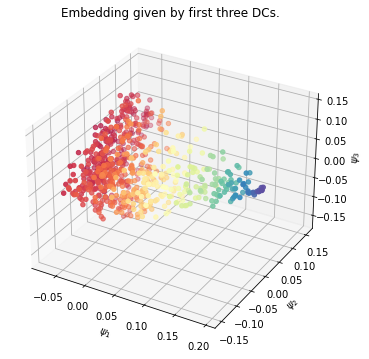
\includegraphics[width=\textwidth]{figures/X1_embedding.png}
    \caption{Three-dimensional embedding of the original point cloud $X_1$.}
\end{subfigure}
\hfill
\begin{subfigure}[b]{0.3\textwidth}
    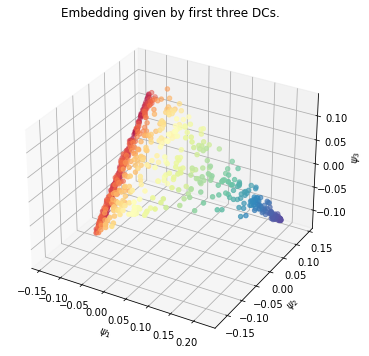
\includegraphics[width=\textwidth]{figures/X2_embedding.png}
    \caption{Three-dimensional embedding of the original point cloud $X_2$.}
\end{subfigure}
\hfill
\begin{subfigure}[b]{0.3\textwidth}
    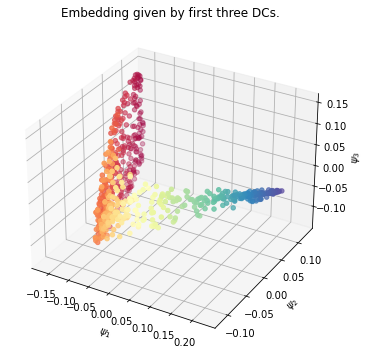
\includegraphics[width=\textwidth]{figures/X3_embedding.png}
    \caption{Three-dimensional embedding of the original point cloud $X_3$.}
\end{subfigure}
\hfill
\begin{subfigure}[b]{0.3\textwidth}
    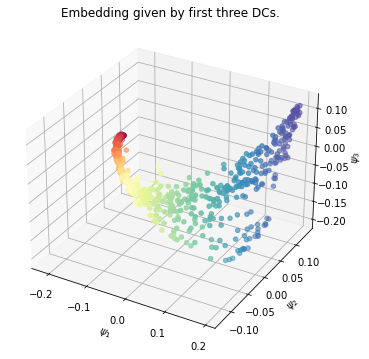
\includegraphics[width=\textwidth]{figures/X4_embedding.png}
    \caption{Three-dimensional embedding of the original point cloud $X_4$.}
\end{subfigure}
\hfill
\begin{subfigure}[b]{0.3\textwidth}
    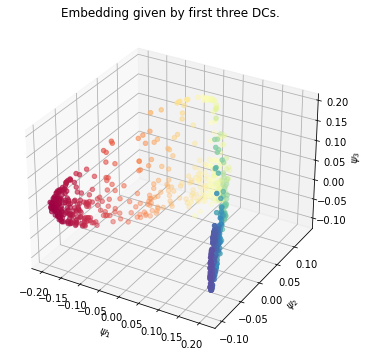
\includegraphics[width=\textwidth]{figures/X5_embedding.png}
    \caption{Three-dimensional embedding of the original point cloud $X_5$.}
\end{subfigure}
\hfill
\begin{subfigure}[b]{0.3\textwidth}
    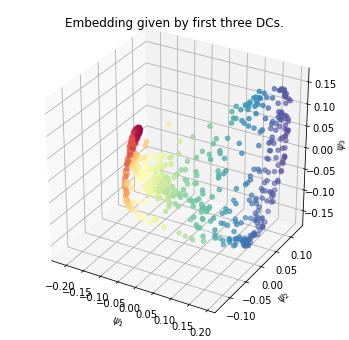
\includegraphics[width=\textwidth]{figures/X6_embedding.png}
    \caption{Three-dimensional embedding of the original point cloud $X_6$.}
\end{subfigure}
\end{figure}

\section{Step 2: Persistent Homology}

Having obtained the three-dimensional embeddings of the point clouds corresponding to six stimuli types, we applied persistent homology to extract the topological features from the six embeddings respectively. In this step, these topological features are represented by persistence barcodes and persistence diagrams.

Our implementation used the package ripser (\cite{ctralie2018ripser}) to obtain the respective persistence diagrams from the embeddings. Using the (birth, death)-intervals from each persistence diagram, we drew the equivalent persistence barcode representation. The complete code can be found in Appendix \ref{AppendixA}. The following figures show the results from applying persistent homology.
\begin{figure}[H]
\centering
\begin{subfigure}[b]{0.2\textwidth}
    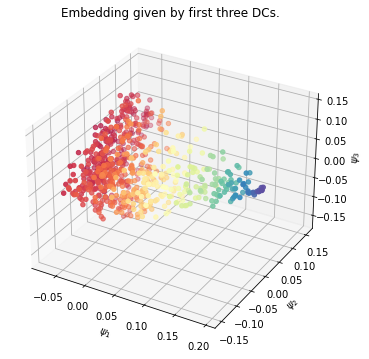
\includegraphics[width=\textwidth]{figures/X1_embedding.png}
    \caption{Three-dimensional embedding of point cloud $X_1$.}
\end{subfigure}
\hfill
\begin{subfigure}[b]{0.75\textwidth}
    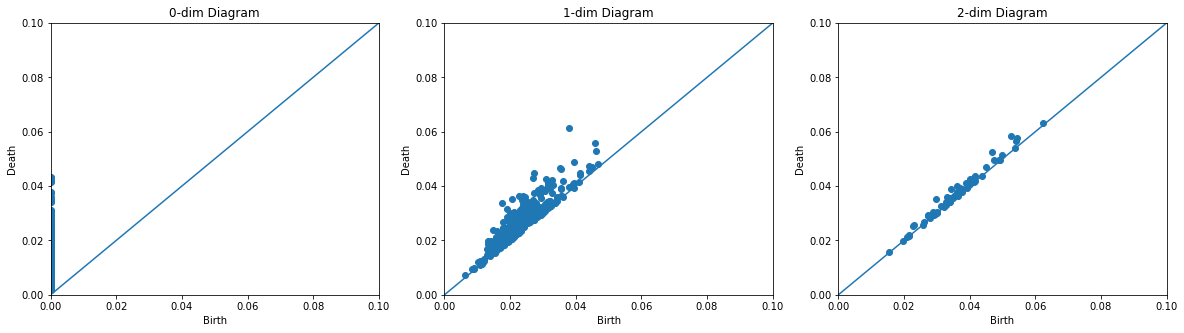
\includegraphics[width=\textwidth]{figures/X1_H0.png}
    \caption*{Persistence diagrams.}
\end{subfigure}
\begin{subfigure}[b]{0.25\textwidth}

\includegraphics[width=\textwidth]{figures/white.png} 
\end{subfigure}
\begin{subfigure}[b]{0.24\textwidth}
    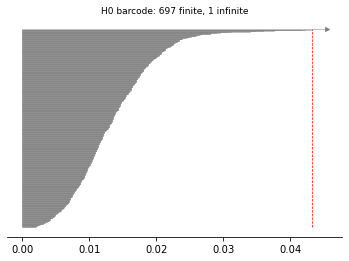
\includegraphics[width=\textwidth]{figures/X1_H0_barcode.png}
    \captionsetup{labelformat=empty}
    \caption{}
\end{subfigure}
\begin{subfigure}[b]{0.24\textwidth}
    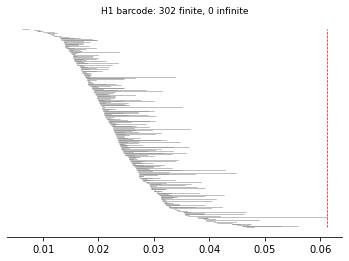
\includegraphics[width=\textwidth]{figures/X1_H1_barcode.png}
        \caption*{Persistence barcodes.}
\end{subfigure}
\begin{subfigure}[b]{0.24\textwidth}
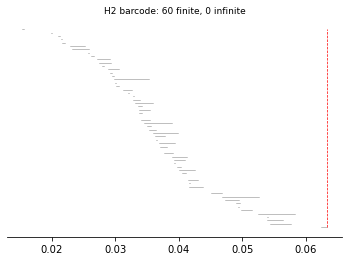
\includegraphics[width=\textwidth]{figures/X1_H2_barcode.png}
\captionsetup{labelformat=empty}
    \caption{}
\end{subfigure}
\caption{Results for applying persistent homology on the three-dimensional embedding of $X_1$.}
\end{figure}

\begin{figure}[H]
\centering
\begin{subfigure}[b]{0.2\textwidth}
    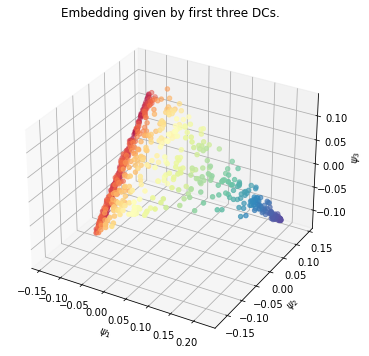
\includegraphics[width=\textwidth]{figures/X2_embedding.png}
    \caption{Three-dimensional embedding of the original point cloud $X_2$.}
\end{subfigure}
\hfill
\begin{subfigure}[b]{0.75\textwidth}
    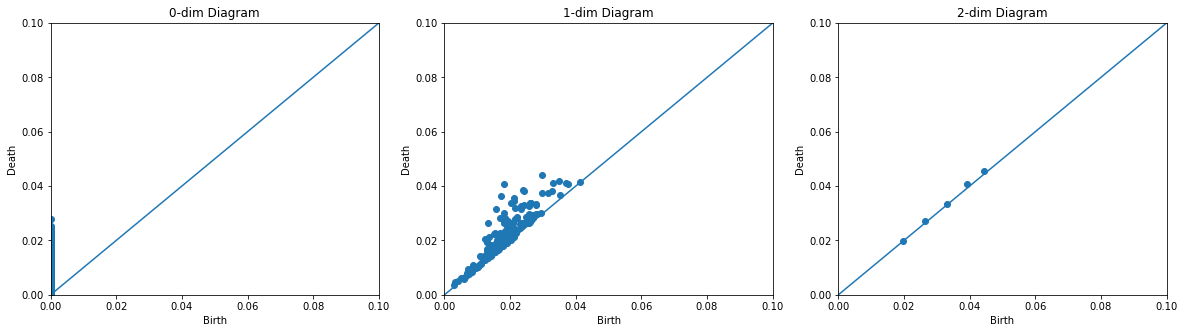
\includegraphics[width=\textwidth]{figures/X2_H0.png}
    \caption{Persistence diagrams.}
\end{subfigure}
\begin{subfigure}[b]{0.25\textwidth}

\includegraphics[width=\textwidth]{figures/white.png} 
\end{subfigure}
\begin{subfigure}[b]{0.24\textwidth}
    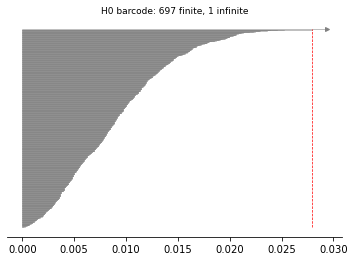
\includegraphics[width=\textwidth]{figures/X2_H0_barcode.png}
    \caption{}
\end{subfigure}
\begin{subfigure}[b]{0.24\textwidth}
    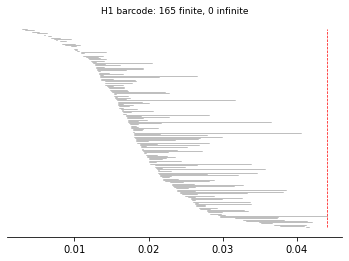
\includegraphics[width=\textwidth]{figures/X2_H1_barcode.png}
        \caption{Persistence barcodes.}
\end{subfigure}
\begin{subfigure}[b]{0.24\textwidth}
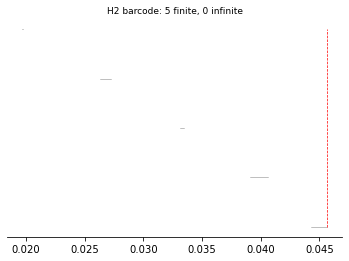
\includegraphics[width=\textwidth]{figures/X2_H2_barcode.png}
 \caption{}
\end{subfigure}
\caption{Results for applying persistent homology on the three-dimensional embedding of $X_2$.}
\end{figure}

\begin{figure}[H]
\centering
\begin{subfigure}[b]{0.2\textwidth}
    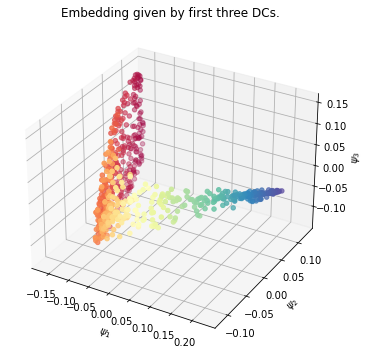
\includegraphics[width=\textwidth]{figures/X3_embedding.png}
    \caption{Three-dimensional embedding of the original point cloud $X_3$.}
\end{subfigure}
\hfill
\begin{subfigure}[b]{0.75\textwidth}
    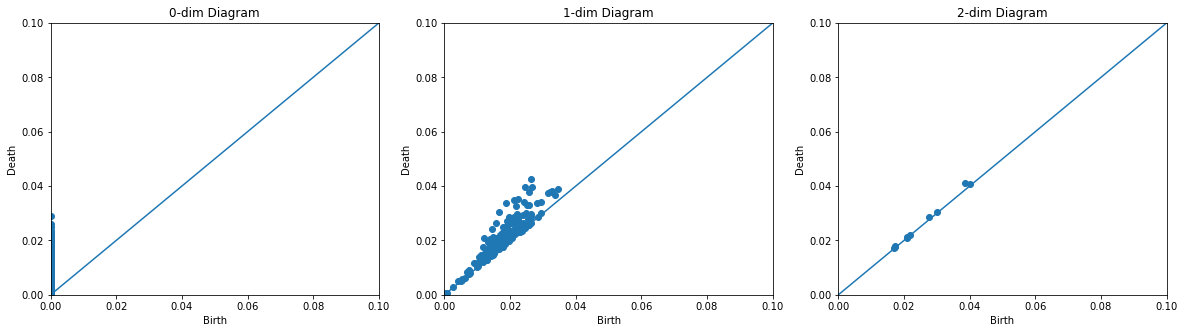
\includegraphics[width=\textwidth]{figures/X3_H0.png}
    \caption{Persistence diagrams.}
\end{subfigure}
\begin{subfigure}[b]{0.25\textwidth}

\includegraphics[width=\textwidth]{figures/white.png} 
\end{subfigure}
\begin{subfigure}[b]{0.24\textwidth}
    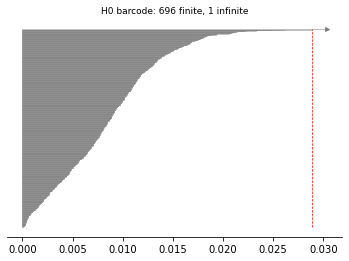
\includegraphics[width=\textwidth]{figures/X3_H0_barcode.png}
    \caption{}
\end{subfigure}
\begin{subfigure}[b]{0.24\textwidth}
    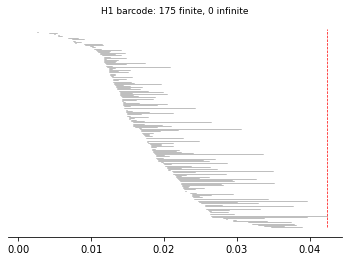
\includegraphics[width=\textwidth]{figures/X3_H1_barcode.png}
        \caption{Persistence barcodes.}
\end{subfigure}
\begin{subfigure}[b]{0.24\textwidth}
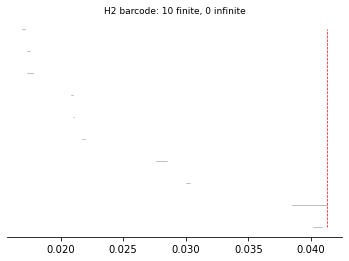
\includegraphics[width=\textwidth]{figures/X3_H2_barcode.png}
 \caption{}
\end{subfigure}
\caption{Results for applying persistent homology on the three-dimensional embedding of $X_3$.}
\end{figure}

\begin{figure}[H]
\centering
\begin{subfigure}[b]{0.2\textwidth}
    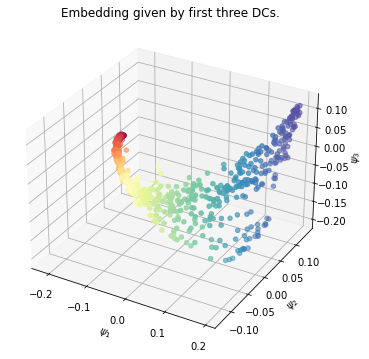
\includegraphics[width=\textwidth]{figures/X4_embedding.png}
    \caption{Three-dimensional embedding of the original point cloud $X_4$.}
\end{subfigure}
\hfill
\begin{subfigure}[b]{0.75\textwidth}
    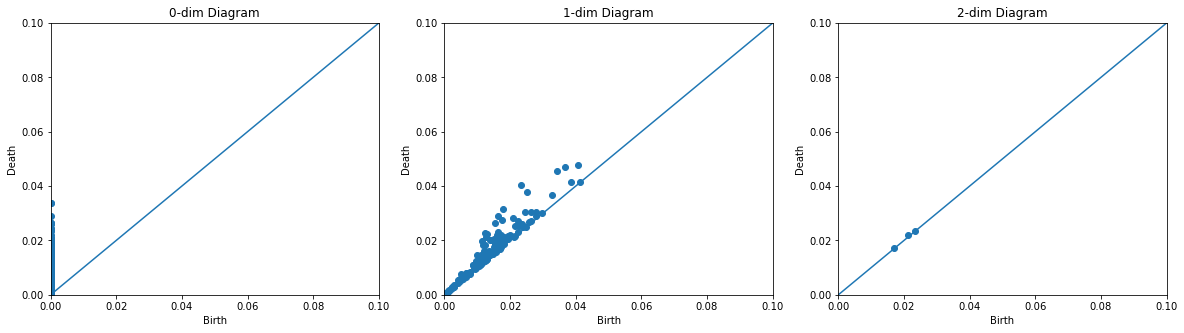
\includegraphics[width=\textwidth]{figures/X4_H0.png}
    \caption{Persistence diagrams.}
\end{subfigure}
\begin{subfigure}[b]{0.25\textwidth}

\includegraphics[width=\textwidth]{figures/white.png} 
\end{subfigure}
\begin{subfigure}[b]{0.24\textwidth}
    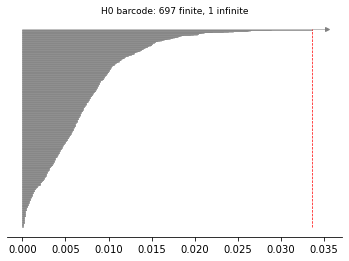
\includegraphics[width=\textwidth]{figures/X4_H0_barcode.png}
    \caption{}
\end{subfigure}
\begin{subfigure}[b]{0.24\textwidth}
    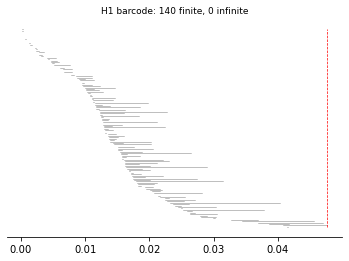
\includegraphics[width=\textwidth]{figures/X4_H1_barcode.png}
        \caption{Persistence barcodes.}
\end{subfigure}
\begin{subfigure}[b]{0.24\textwidth}
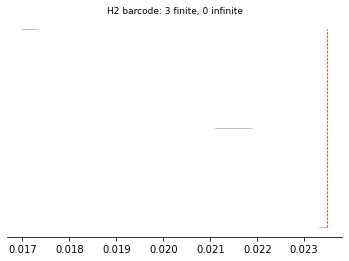
\includegraphics[width=\textwidth]{figures/X4_H2_barcode.png}
 \caption{}
\end{subfigure}
\caption{Results for applying persistent homology on the three-dimensional embedding of $X_4$.}
\end{figure}

\begin{figure}[H]
\centering
\begin{subfigure}[b]{0.2\textwidth}
    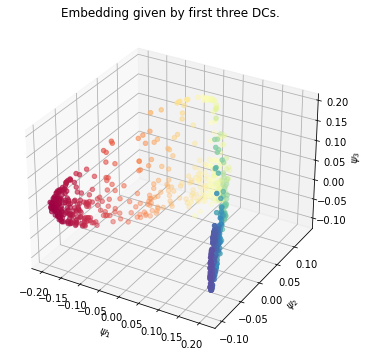
\includegraphics[width=\textwidth]{figures/X5_embedding.png}
    \caption{Three-dimensional embedding of the original point cloud $X_5$.}
\end{subfigure}
\hfill
\begin{subfigure}[b]{0.75\textwidth}
    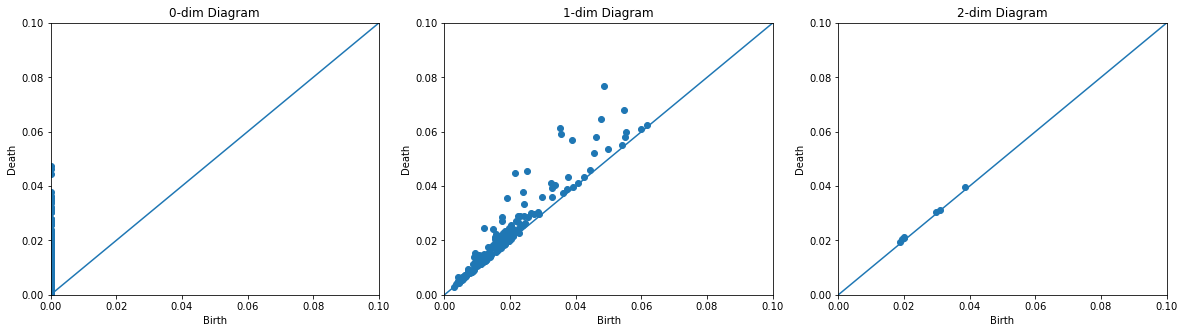
\includegraphics[width=\textwidth]{figures/X5_H0.png}
    \caption{Persistence diagrams.}
\end{subfigure}
\begin{subfigure}[b]{0.25\textwidth}

\includegraphics[width=\textwidth]{figures/white.png} 
\end{subfigure}
\begin{subfigure}[b]{0.24\textwidth}
    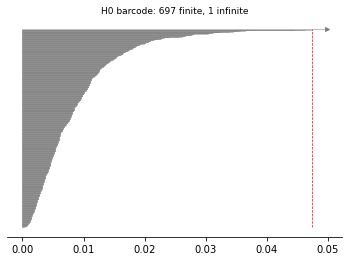
\includegraphics[width=\textwidth]{figures/X5_H0_barcode.png}
    \caption{}
\end{subfigure}
\begin{subfigure}[b]{0.24\textwidth}
    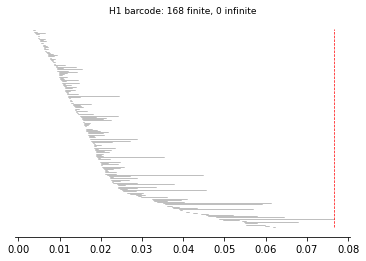
\includegraphics[width=\textwidth]{figures/X5_H1_barcode.png}
        \caption{Persistence barcodes.}
\end{subfigure}
\begin{subfigure}[b]{0.24\textwidth}
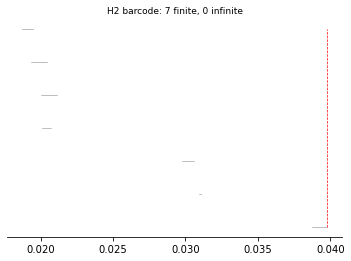
\includegraphics[width=\textwidth]{figures/X5_H2_barcode.png}
 \caption{}
\end{subfigure}
\caption{Results for applying persistent homology on the three-dimensional embedding of $X_5$.}
\end{figure}

\begin{figure}[H]
\centering
\begin{subfigure}[b]{0.2\textwidth}
    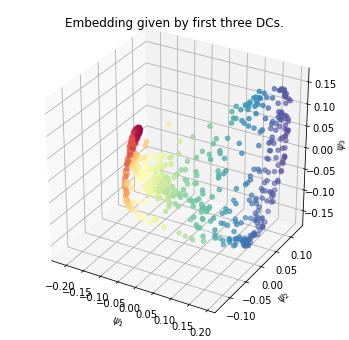
\includegraphics[width=\textwidth]{figures/X6_embedding.png}
    \caption{Three-dimensional embedding of the original point cloud $X_6$.}
\end{subfigure}
\hfill
\begin{subfigure}[b]{0.75\textwidth}
    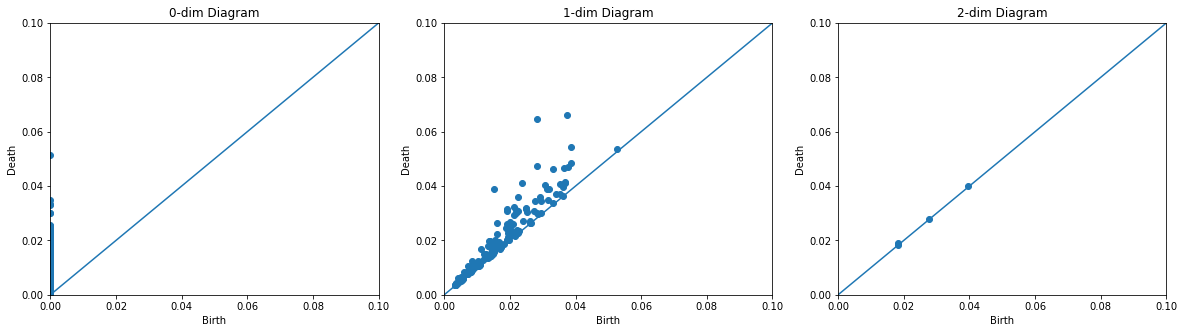
\includegraphics[width=\textwidth]{figures/X6_H0.png}
    \caption{Persistence diagrams.}
\end{subfigure}
\begin{subfigure}[b]{0.25\textwidth}

\includegraphics[width=\textwidth]{figures/white.png} 
\end{subfigure}
\begin{subfigure}[b]{0.24\textwidth}
    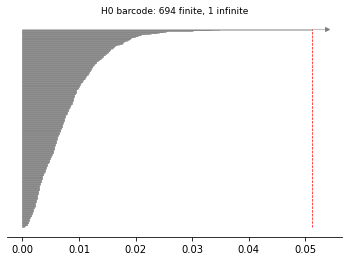
\includegraphics[width=\textwidth]{figures/X6_H0_barcode.png}
    \caption{}
\end{subfigure}
\begin{subfigure}[b]{0.24\textwidth}
    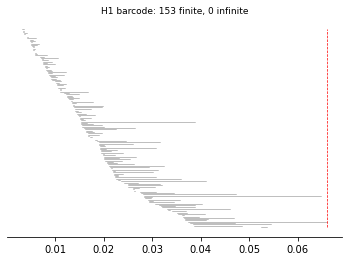
\includegraphics[width=\textwidth]{figures/X6_H1_barcode.png}
        \caption{Persistence barcodes.}
\end{subfigure}
\begin{subfigure}[b]{0.24\textwidth}
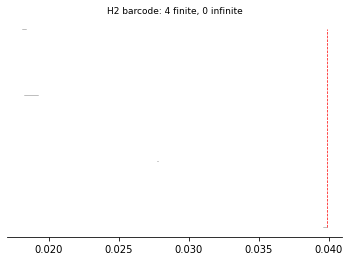
\includegraphics[width=\textwidth]{figures/X6_H2_barcode.png}
 \caption{}
\end{subfigure}
\caption{Results for applying persistent homology on the three-dimensional embedding of $X_6$.}
\end{figure}

\section{Step 3: Pairwise Wasserstein distance}
In the last step, we used the gudhi package (\cite{gudhi:urm}) to compute the pairwise Wasserstein distance between the persistence diagrams. The method used is based on (\cite{kerber_geometry_2016}). 

We first computed the first pairwise distances between the persistence diagrams for each of the six point clouds. 

\begin{table}[!htbp]
        \centering
        \small
        \setlength\tabcolsep{5pt}
        \begin{tabular}{|c|c|c|c|c|c|c|}
\hline
 $H_0$& $X_1$ & $X_2$ & $X_3$ & $X_4$ & $X_5$ & $X_6$\\
 \hline
$X_1$ &
0.0&
\textbf{2.77}&
\textbf{3.05}&
\textbf{3.95}&
\textbf{3.08}&
\textbf{3.42}
\\
\hline
$X_2$ &
\textbf{2.77}&
0.0&
0.43&
1.35&
1.0&
0.84
\\
\hline
$X_3$ &
\textbf{3.05}&
0.43&
0.0&
1.03&
0.94&
0.66
\\
\hline
$X_4$ &
\textbf{3.95}&
1.35&
1.03&
0.0&
1.11&
0.72
\\
\hline
$X_5$ &
\textbf{3.08}&
1.0&
0.94&
1.11&
0.0&
0.51
\\
\hline
$X_6$ &
\textbf{3.42}&
0.84&
0.66&
0.72&
0.51&
0.0
\\
\hline
\end{tabular}
\caption{Pairwise Wasserstein distance between persistent diagrams for homology group $H_0$.}
\label{tab:Wass_H0}
\end{table}

\begin{table}[!htbp]
        \centering
        \small
        \setlength\tabcolsep{5pt}
        \begin{tabular}{|c|c|c|c|c|c|c|}
\hline
 $H_1$& $X_1$ & $X_2$ & $X_3$ & $X_4$ & $X_5$ & $X_6$ \\ \hline
$X_1$ &
0.0&
0.46&
0.5&
0.64&
0.64&
0.55

\\\hline
$X_2$ &
0.46&
0.0&
0.17&
0.29&
0.36&
0.3
\\\hline
$X_3$ &
0.5&
0.17&
0.0&
0.25&
0.33&
0.3
\\\hline 
$X_4$ &
0.64&
0.29&
0.25&
0.0&
0.27&
0.29
\\\hline 
$X_5$ &
0.64&
0.36&
0.33&
0.27&
0.0&
0.26

\\\hline
$X_6$ &
0.55&
0.3&
0.3&
0.29&
0.26&
0.0\\
\hline
\end{tabular}
\caption{Pairwise Wasserstein distance between persistent diagrams for homology group $H_1$.}
\label{tab:Wass_H1}
\end{table}

\begin{table}[!htbp]
        \centering
        \small
        \setlength\tabcolsep{5pt}
        \begin{tabular}{|c|c|c|c|c|c|c|}
\hline
 $H_2$& $X_1$ & $X_2$ & $X_3$ & $X_4$ & $X_5$ & $X_6$ \\ \hline
$X_1$ &
0.0&
0.06&
0.06&
0.06&
0.06&
0.06
\\
\hline
$X_2$ &
0.06&
0.0&
0.01&
0.0&
0.01&
0.0
\\
\hline
$X_3$ &
0.06&
0.01&
0.0&
0.0&
0.01&
0.0
\\
\hline
$X_4$ &
0.06&
0.0&
0.0&
0.0&
0.0&
0.0
\\
\hline
$X_5$ &
0.06&
0.01&
0.01&
0.0&
0.0&
0.0
\\
\hline
$X_6$ &
0.06&
0.0&
0.0&
0.0&
0.0&
0.0
\\
\hline
\end{tabular}
\caption{Pairwise Wasserstein distance between persistent diagrams for homology group $H_2$.}
\label{tab:Wass_H2}
\end{table}

Building upon the same method, we further compared the six point clouds with known three-dimensional shapes ($2$-sphere and torus) based on the Wasserstein distance.

First, we extracted the topological features of the $2$-sphere and three-dimensional torus, as we did for the point clouds in Step 2. 
\begin{figure}[H]
\centering
\begin{subfigure}[b]{0.2\textwidth}
    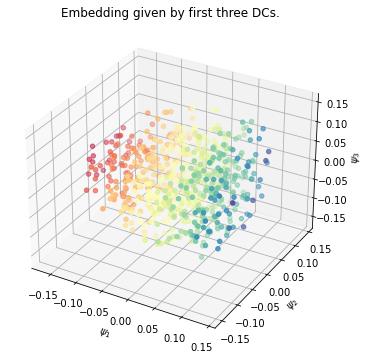
\includegraphics[width=\textwidth]{figures/dsphere.png}
    \caption{Scatter plot for $2$-sphere.}
\end{subfigure}
\hfill
\begin{subfigure}[b]{0.75\textwidth}
    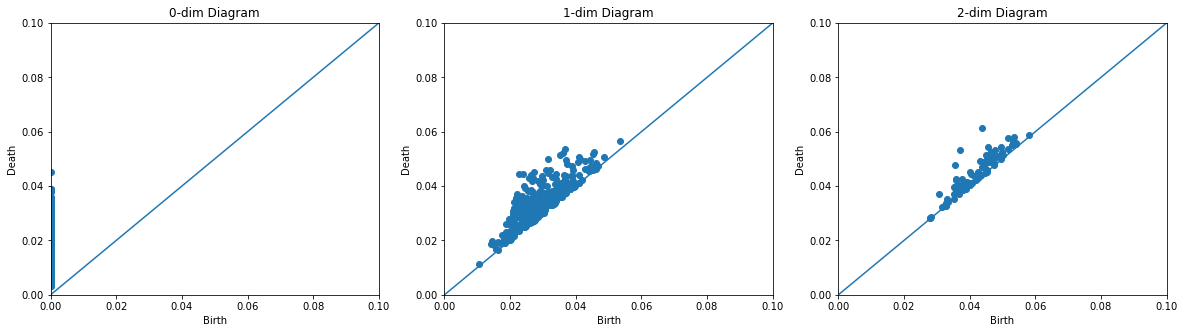
\includegraphics[width=\textwidth]{figures/dsphere_Hk.png}
    \caption{Persistence diagrams.}
\end{subfigure}
\begin{subfigure}[b]{0.25\textwidth}

\includegraphics[width=\textwidth]{figures/white.png} 
\end{subfigure}
\begin{subfigure}[b]{0.24\textwidth}
    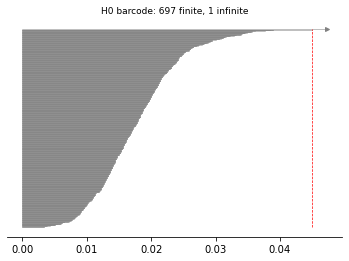
\includegraphics[width=\textwidth]{figures/dsphere_H0_barcode.png}
    \caption{}
\end{subfigure}
\begin{subfigure}[b]{0.24\textwidth}
    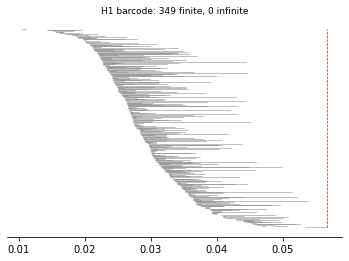
\includegraphics[width=\textwidth]{figures/dsphere_H1_barcode.png}
        \caption{Persistence barcodes.}
\end{subfigure}
\begin{subfigure}[b]{0.24\textwidth}
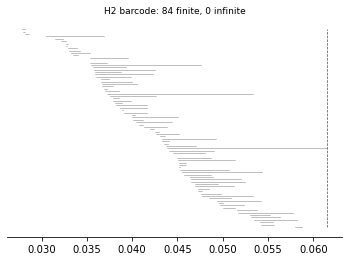
\includegraphics[width=\textwidth]{figures/dsphere_H2_barcode.png}
 \caption{}
\end{subfigure}
\caption{Results for applying persistent homology on the $2$-sphere.}
\end{figure}

\begin{figure}[H]
\centering
\begin{subfigure}[b]{0.2\textwidth}
    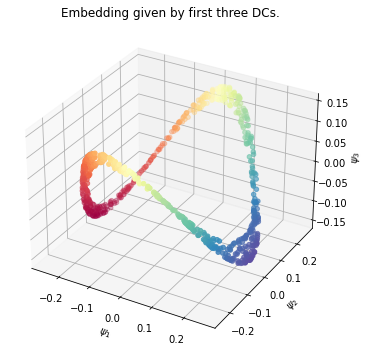
\includegraphics[width=\textwidth]{figures/torus.png}
    \caption{Scatter plot for the three-dimensional torus.}
\end{subfigure}
\hfill
\begin{subfigure}[b]{0.75\textwidth}
    \includegraphics[width=\textwidth]{figures/torus_Hk.png}
    \caption{Persistence diagrams.}
\end{subfigure}
\begin{subfigure}[b]{0.25\textwidth}
\includegraphics[width=\textwidth]{figures/white.png} 
\end{subfigure}
\begin{subfigure}[b]{0.24\textwidth}
    \includegraphics[width=\textwidth]{figures/torus_H0_barcode.png}
    \caption{}
\end{subfigure}
\begin{subfigure}[b]{0.24\textwidth}
    \includegraphics[width=\textwidth]{figures/torus_H1_barcode.png}
        \caption{Persistence barcodes.}
\end{subfigure}
\begin{subfigure}[b]{0.24\textwidth}
\includegraphics[width=\textwidth]{figures/torus_H2_barcode.png}
 \caption{}
\end{subfigure}
\caption{Results for applying persistent homology on the three-dimensional torus.}
\end{figure}

Then, we computed the Wasserstein distance between the six point clouds and the known shapes:

\begin{table}[!htbp]
        \centering
        \small
        \setlength\tabcolsep{5pt}
        \begin{tabular}{|c|c|c|c|c|c|c|}
\hline
  $H_0$& $X_1$ & $X_2$ & $X_3$ & $X_4$ & $X_5$ & $X_6$ \\ \hline
$2$-sphere & 2.48 & 4.46&  4.64 & 5.18 & 4.53 & 4.83\\\hline
torus & 3.63 &  1.46 & 1.31 & 0.73 & 1.38 & 1.06 \\ \hline
\end{tabular}
\caption{Wasserstein distance between persistent diagrams of the point clouds and $2$-sphere and torus (homology group $H_0$).}
\label{tab:sphere-H0}
\end{table}


\begin{table}[!htbp]
        \centering
        \small
        \setlength\tabcolsep{5pt}
        \begin{tabular}{|c|c|c|c|c|c|c|}
\hline
$H_1$& $X_1$ & $X_2$ & $X_3$ & $X_4$ & $X_5$ & $X_6$ \\ \hline
$2$-sphere & 0.62 &   0.77 & 0.80 & 0.87 & 0.85 & 0.76\\\hline
torus & 0.74 & 0.49 & 0.44 & 0.34 & 0.45 & 0.47\\ \hline
\end{tabular}
\caption{Wasserstein distance between persistent diagrams of the point clouds and $2$-sphere and torus (homology group $H_1$).}
\label{tab:sphere-H1}
\end{table}

\begin{table}[!htbp]
        \centering
        \small
        \setlength\tabcolsep{5pt}
        \begin{tabular}{|c|c|c|c|c|c|c|}
\hline
$H_2$ & $X_1$ & $X_2$ & $X_3$ & $X_4$ & $X_5$ & $X_6$ \\ \hline
$2$-sphere & 0.11 &   0.12 & 0.12 & 0.12 & 0.13 & 0.12\\\hline
torus & 0.057 & 0.017 & 0.018  & 0.016 & 0.018 & 0.016 \\ \hline
\end{tabular}
\caption{Wasserstein distance between persistent diagrams of the point clouds and $2$-sphere and torus (homology group $H_2$).}
\label{tab:sphere-H2}
\end{table}

\section{Analysis of results}
Based on the results from the above tables of Wasserstein distances, our observations and inferences are as follows.

\begin{enumerate}
    \item The topological structure for $X_1$ is distinct from the rest. 
    
    Based on the pairwise Wasserstein distances in Tables \ref{tab:Wass_H0} and \ref{tab:Wass_H1}, $X_1$ is notably different from the rest of the point clouds in terms of topological structure. In the context of our application, this implies that the neural population response evoked by stimulus type 1 is significantly different from the other stimulus types. This observation leads us to hypothesize that there is some neuroscientific reason behind this distinction in the topological structure of neural population response. It might be interesting to conduct further lab experiments to investigate what special properties this stimulus has and why it causes such different  neural population response. 
    
    \item Wasserstein distances between persistence diagrams are nearly negligible for $H_2$.
    
    Based on Table \ref{tab:Wass_H2}, pairwise Wasserstein distances between persistence diagrams for $H_2$ are small enough to be nearly negligible. This implies that the intrinsic dimensionality of this neural data might be even lower than three-dimensional since there is no significant differences in homology groups $H_2$ for the point clouds.
    
    \item Shape comparison with $2$-sphere and torus.
    
    Based on Tables \ref{tab:sphere-H0} and \ref{tab:sphere-H1}, the Wasserstein distances between the point clouds and the $2$-sphere are smaller than the Wasserstein distances between the point clouds and the torus for all $X_i$ except for $X_1$. We can thus infer that except for $X_1$, all other point clouds are more similar to the shape of a torus than the $2$-sphere. This implies that the topological structure of the neural population response evoked by stimuli type 1 is more similar to a sphere while the neural population response evoked by the rest of the stimuli types used in the experiments are more similar to a torus. 
    
    It would be interesting to compare this result with the hypothesis in (\cite{ben-yishai_theory_1995}, \cite{Blumenfeld_2006}, \cite{goldberg_randomized_2004},    \cite{singh_top_v1_2008}):
    If we are given an oriented stimulus, and if the orientation is a circular variable, then the hypothesis is that the neural population response evoked by such stimulus must have a topological structure equivalent to that of a circle. However, to fully test this hypothesis, further experiments with different types of stimuli need to be conducted.
\end{enumerate}

\section{Conclusion}
In this chapter, we demonstrated our proposed approach to compare the point clouds that represent the neural population response to different stimuli. Our proposed approach is contingent on the topological structures of the point clouds.  

One significant limitation in this specific application is that lab data usually involve a lot of sampling errors such as missing data and inconsistent densities, causing noise to the true underlying geometry of the neural population response. Persistent homology works well on synthetic data, but might not work when the sampling errors are too significant.

The advantages of topological approach is that we can provide a succinct and useful summary of the global geometric structure of the neural spiking data, thus obtaining a useful account of how similarly the neurons collectively respond to visual stimuli. This is especially important in applications where the notion of connectedness and clusters are salient. As an emerging field, TDA will certainly see more applications in solving problems that involve understanding the geometric and topological structure of high-dimensional data.